Anonymous marketplaces are a rapidly growing segment of online illegal drug
sales. Figures \ref{agora} and \ref{product_time} show the mainstream user
interface and product listing growth of one such site.
However, due to their clandestine nature, it can be difficult to extract information about product listings without manual intervention.
Law enforcement officials and interested researchers must have an expert manually tag each listing or rely on error prone ad-hoc methods of catagorizing product listings.

To improve this process, we developed a machine learning algorithm that can
automatically categorize listings with high accuracy. The input to our algorithm
is the listing text, including it's title and description. We then use TF-IDF to
extract features followed by PCA to select features from the text.  Finally, we
use a SVM to classifiy the features and output a product category.

All data processing and machine learning was executed using tools and algorithms
in scikit-learn \cite{scikit-learn}. Plots were generated using matplotlib
\cite{matplotlib}.
\begin{figure}[htbp]
    \begin{minipage}[t]{0.45\linewidth}
        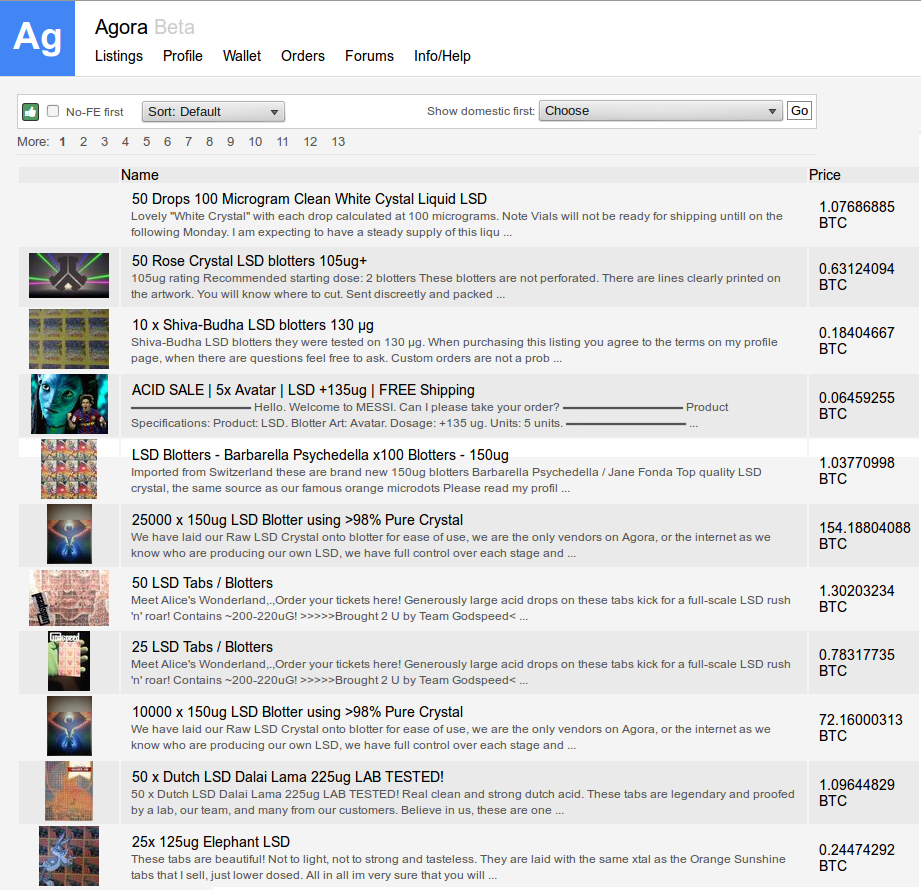
\includegraphics[width=\linewidth]{agora}
        \caption{Agora Marketplace on January 2015}
        \label{agora}
    \end{minipage}
    \hfill
    \begin{minipage}[t]{0.45\linewidth}
        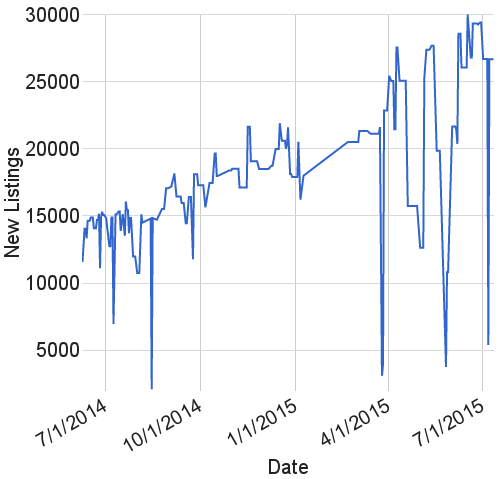
\includegraphics[width=\linewidth]{plots/new_listings_graph}
        \caption{New Product Listings Over Time}
        \label{product_time}
    \end{minipage}
\end{figure}
